%%https://rpubs.com/davoodastaraky/mtRegression

%http://rstudio-pubs-static.s3.amazonaws.com/20516_29b941670a4b42688292b4bb892a660f.html

In this Chapter we finally get our hands dirty with some real data! After learning how to acquire and import data, here we put that all in practice in our first data analysis case. This chapter is very hands-on, so we will present a complete and self-contained data science problem\footnote{See the works of Ryan Quan and Davood Astaraky for further reference}. We break down our investigation into small pieces. First, we have a quick look at our data, to then explore it in more detail. Finally, we design a numerical model to estimate some features of our dataset. 

\section{Descriptive data analysis}\label{initDA}

The case we present here is a classic one. We want to know if cars with a manual transmission are more fuel efficient than automatic-transmission cars. Following our methodology we first define our research questions. In this case, they are:
 
\begin{itemize}
\item Is there a difference in miles per gallon (MPG) between automatic and manual transmission cars?
\item Can we quantify the difference?
\end{itemize}

The data was extracted from the 1974 Motor Trend US magazine. It is called (\textit{mtcars}) and it comprises fuel consumption and 10 other aspects of car design and performance for 32 cars (73–74 models). Let's have a good look at what variables we have available, first:

\begin{figure}[ht]
	\begin{center}
			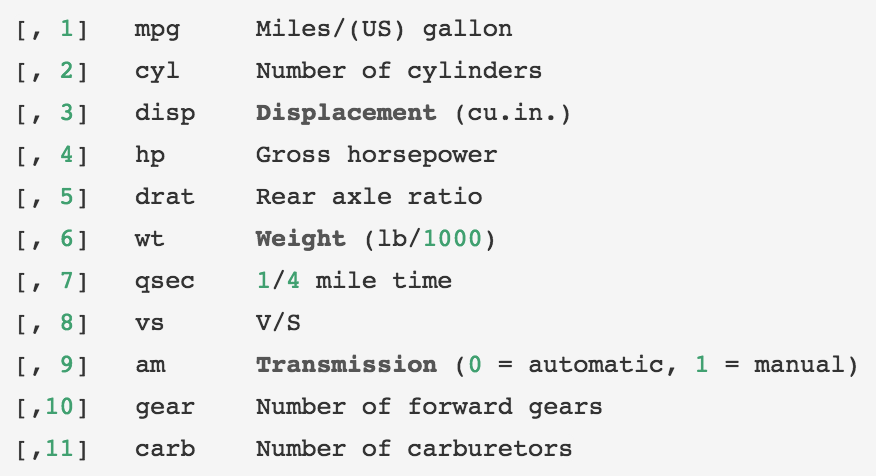
\includegraphics[scale=0.6]{Parts/numerics/desc1}
	\end{center}
	\caption{List of variables present in the mtcars dataset.}
	\label{fig:desc1}
\end{figure}

Also the first six records of the dataset are shown below:

\begin{figure}[ht]
	\begin{center}
			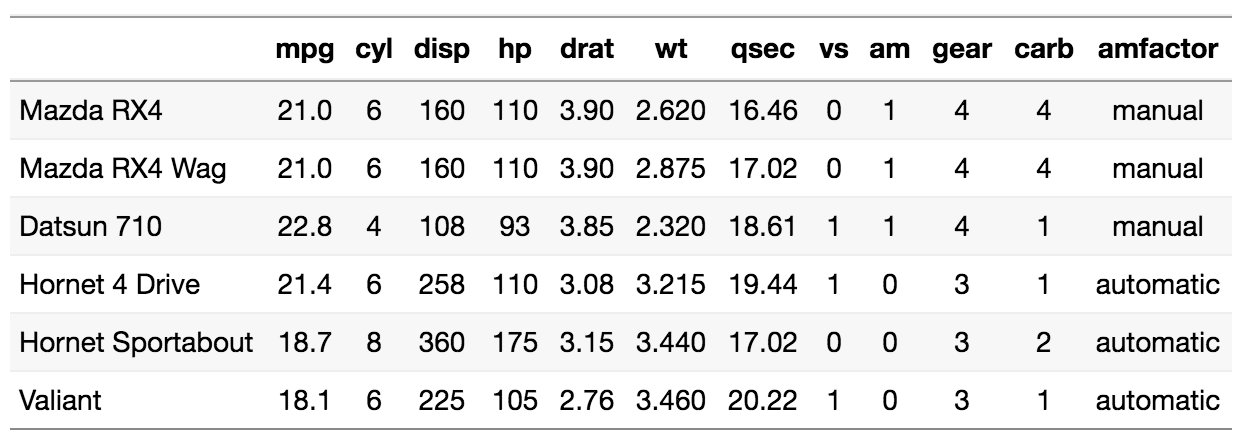
\includegraphics[scale=0.5]{Parts/numerics/desc2}
	\end{center}
	\caption{Six complete records. Every row represents a unique car model. The attributes names are described in Fig. \ref{fig:desc1}}
	\label{fig:desc2}
\end{figure}

\section{Exploratory data analysis}\label{ExpDA}

After this quick summary it is time to explore the dataset. Let's begin by looking at the MPG frequency distribution. \newpage

\begin{figure}[ht]
	\begin{center}
			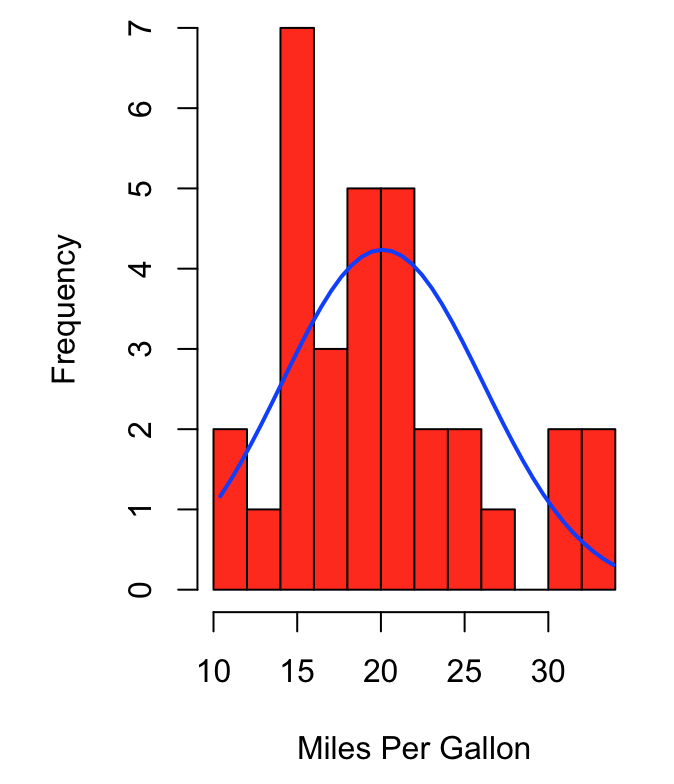
\includegraphics[scale=0.5]{Parts/numerics/hist1}
	\end{center}
	\caption{Frequency distribution of MPG}
	\label{fig:hist1}
\end{figure}

We observe that the MPG distribution falls more or less under the normal curve (blue). Moreover, there are no apparent outliers. The whole range is contained within 10-35 MPG. That's good news for us! We can now plot the MPG for automatic and manual cars separately. What plot is better than a box-plot in this case?

\begin{figure}[ht]
	\begin{center}
			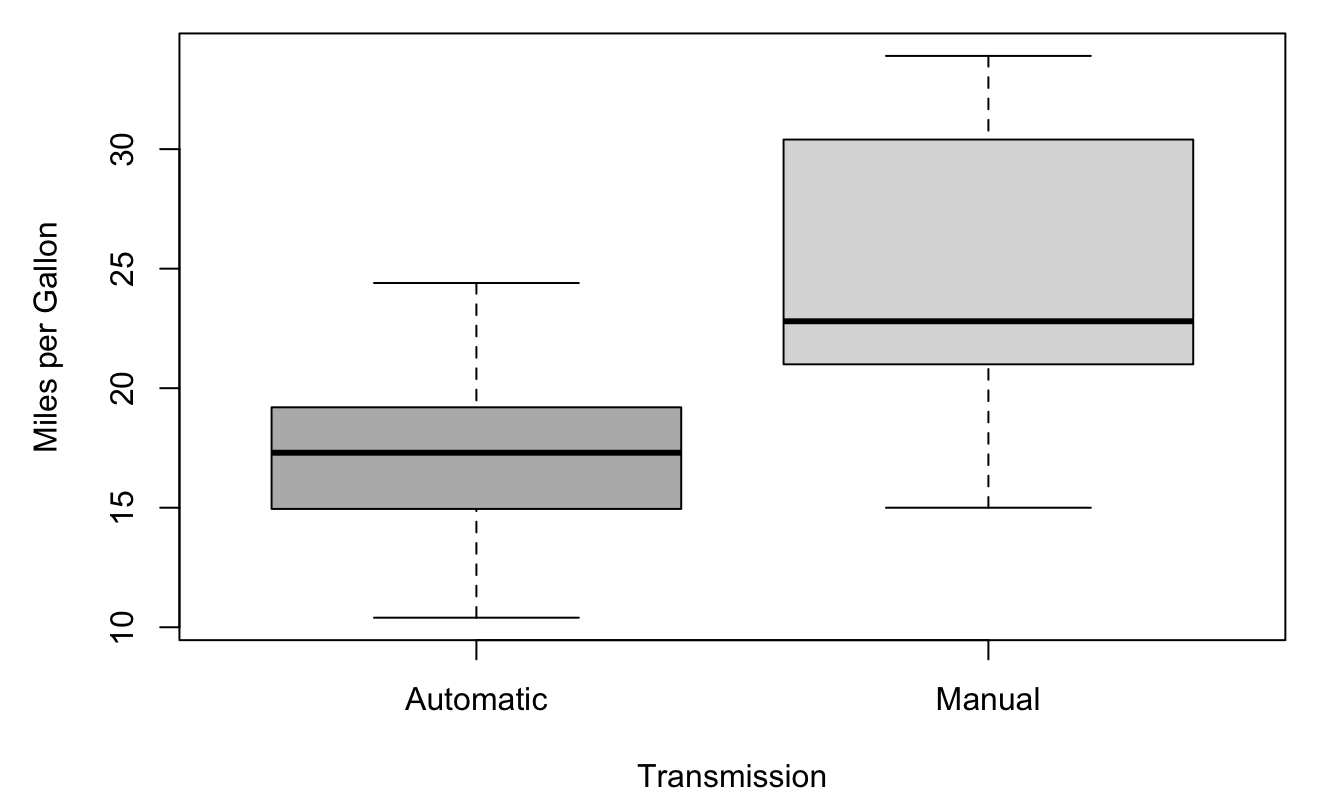
\includegraphics[scale=0.35]{Parts/numerics/bplot1}
	\end{center}
	\caption{MPG by transmission type}
	\label{fig:bplot1}
\end{figure}

Indeed, as shown in Fig. \ref{fig:hist1} the range which the MPG is distributed lies within 10-35. However, the box-plot separates the manual from automatic cars, allowing us to see that there is a (big?) difference between the two classes. Apparently, automatic cars have a lower MPG, following common sense. The medians are 17 and 23 MPG for automatic and manual, respectively. In addition, 50$\%$ of the automatic cars have an MPG confined within the range 15-20 MPG. This range is somewhat wider for manual cars ($\approx$ 20-30 MPG). Now, we have to prove that the difference we observe is not due to random chance, i.e. we just picked a bunch of automatic cars that not efficient and compared to very efficient manual cars. To make sure that does not happen we can use a statistical test. Here, we will use the so-called ``two Sample t-test''. 

The results are shown below:

\begin{figure}[ht]
	\begin{center}
			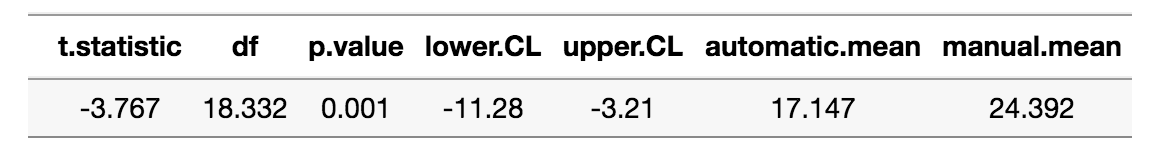
\includegraphics[scale=0.5]{Parts/numerics/ttest}
	\end{center}
%	\caption{}
	\label{fig:ttest}
\end{figure}

This test proves that cars with an automatic transmission use more fuel than cars with a manual transmission. The p-value ($0.001$) shows the probability that this apparent difference could appear by chance. Based on the very p-value the probability is negligible. The confidence intervals (3.2 - 11.3 MPG) describe the range of how much higher is the MPG in automatic cars, if compared to in manual cars.

Now, what if we want to design a model to estimate MPG based on the other variables we have in our dataset?

%https://www.datacamp.com/community/tutorials
%https://www.datacamp.com/community/tutorials/importing-data-r-part-two

\section{Regresion analysis}\label{RegDA}

What is the simplest model we can design? We'd say: what about a linear model that, given the type of transmission (automatic or manual), returns the MPG? Something like:

\begin{equation}
y = ax + b,
\end{equation}

\noindent where ``x'' is the transmission, ``y'' is the consumption in MPG, and ``a'' and ``b'' are numerical coefficients. That sounds simple enough, right? Let's have a look at the results of such linear regression:

\begin{figure}[ht]
	\begin{center}
			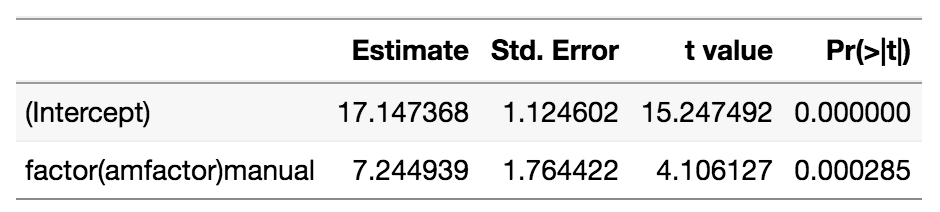
\includegraphics[scale=0.5]{Parts/numerics/linR}
	\end{center}
%	\caption{}
	\label{fig:linR}
\end{figure}

We are somewhat familiar with these numbers already. 17.1 is just the mean for automatic cars and the slope (7.2) is the difference, in MPG, between manual and automatic cars. The p-value is also very small, indicating that there's a significant difference between automatic and manual cars. However, if you calculate the R$^2$ of this fit you will get a very low 0.36. These results, together with the information we already have from the box-plots, make this model a little redundant - besides explaining only 36$\%$ of the variance.

Our previous results are calling for a more robust model. We will try a multi-variate linear model. In order to determine which predictors one should use, we create a correlation matrix for the MPG variable. Do it yourself and you will see that \textit{wt}, \textit{cyl}, \textit{disp}, and \textit{hp} are highly correlated with \textit{MPG} ($\left|0.7\right|$ or higher).

Let's do a full stop here: does that make sense? \textit{wt} and \textit{hp} make very good sense to us; heavier cars and more powerful cars should have lower MPG values. Note, however, that \textit{disp} and \textit{cyl} are highly correlated with each other. Due to that we decided to exclude them from our analysis. Summarizing we are making a model that looks like the following:

\begin{equation}
y = ax_1 + bx_2 + cx_3 + d,
\end{equation}

where $x_1,x_2,x_3$ are $am,wt$, and $hp$ respectively, and $a,b,c$, and $d$ are numerical coefficients to be determined by the model.

Since this Chapter is hands-on we will design this model together. The results are surprising. By introducing \textit{wt} and \textit{hp} to our modelling framework we obtain a R$^2$ of 0.84. This is much higher than $0.36$, obtained with the simple linear regression. This model predicts that, on average, manual transmission cars perform on around 2 MPGs more than automatic transmission cars.

If we come back and answer our research questions. Yes, there's a significant difference between automatic and manual transmission cars. We are also able to quantify this difference: 2 MPG. This is just an example of how thinking and modelling-design walk hand-in-hand. 

In the next Chapter we will dive on some machine learning algorithms and techniques.



